\documentclass[12pt,a4paper]{article}
\usepackage[UTF8]{ctex}
\usepackage{graphicx}
\usepackage{geometry}
\usepackage{ulem}
\usepackage{enumitem}
\usepackage{titlesec}
\usepackage{multicol}
\usepackage[export]{adjustbox}
\usepackage{amsmath}  % 推荐用于更好的数学排版
\usepackage[utf8]{inputenc}
\usepackage{CJKutf8}
\usepackage{fancyhdr}
\usepackage{lastpage}
\usepackage{ulem}
\usepackage{tabularx}
\usepackage{float}

% 页眉页脚设置
\pagestyle{fancy}
\fancyhf{} % 清除所有页眉页脚
% 设置页眉内容
%-==========1. 填写从第二页开始 每页第一行的信息==========-
\fancyhead[C]{
    \makebox[4.5em][c]{实验名称：} \uline{\makebox[14em][c]{电路定律实验验证}} 
    \makebox[2.5em][c]{姓名：} \uline{\makebox[4em][c]{}} 
    \makebox[2.5em][c]{学号：} \uline{\makebox[5em][c]{}}
}%--------------------------------------------------------
\fancyfoot[C]{第 \thepage\ 页，共 \pageref{LastPage} 页}

% 取消页眉和页脚的下划线
\renewcommand{\headrulewidth}{0pt} % 页眉横线粗细设为0
\renewcommand{\footrulewidth}{0pt} % 页脚横线粗细设为0

% 调整页眉高度
\setlength{\headheight}{50pt}

% 设置plain样式（用于第一页）
\fancypagestyle{plain}{
    \fancyhf{} % 清除所有页眉页脚
    \renewcommand{\headrulewidth}{0pt} % 隐藏页眉横线
    \fancyfoot[C]{第 \thepage\ 页，共 \pageref{LastPage} 页} % 保留页脚
}
% 设置页面边距
\geometry{left=2.54cm,right=1.5cm,top=2.54cm,bottom=2.54cm}

% 设置正文字体大小为小四
\renewcommand{\normalsize}{\fontsize{12pt}{16pt}\selectfont}
% 设置章节格式
\titleformat{\section}{\fontsize{16pt}{22pt}\selectfont\bfseries}{\thesection}{1em}{} % 一级标题：三号
\titleformat{\subsection}{\fontsize{15pt}{20pt}\selectfont\bfseries}{\thesubsection}{1em}{} % 二级标题：小三

\begin{document}
\thispagestyle{plain}%第一页使用 plain 样式，而不是默认的 fancy 样式，第一页不再显示页眉
% 标题部分 - 两栏布局
\begin{multicols}{2}
    % 左栏：图片和实验报告标题
    % 左栏：使用空行创建前三行
    \noindent
    ~\\ % 第一行
    ~\\ % 第二行
    ~\\ % 第三行
    \hphantom{占位}% 使用空占位符
    \raisebox{-0.5\baselineskip}% 图片向下移动半行
    {
\includegraphics[width=1.85in,height=0.58in]{ZJU.jpg}}
    \hspace{.5em}% 图片和标题之间的间距
    \raisebox{0pt}[\height][0pt]% 标题底部对齐
    {\textbf{\fontsize{26pt}{30pt}\selectfont 实验报告}}
    
    \columnbreak % 换到右栏
    
    % 右栏：个人信息
    % 右栏：个人信息 - 靠右对齐 
%-==========2. 填写个人信息==========-
    \begin{flushright}
        \makebox[3em][l]{专业：} \uline{\makebox[9em][c]{法语-电子科学与技术}} \\
        \makebox[3em][l]{姓名：} \uline{\makebox[9em][c]{}} \\ 
        \makebox[3em][l]{学号：} \uline{\makebox[9em][c]{}} \\
        \makebox[3em][l]{日期：} \uline{\makebox[9em][c]{2025年11月11日}} \\
        \makebox[3em][l]{地点：} \uline{\makebox[9em][c]{紫金港东四216}} \\
    \end{flushright}   
\end{multicols}
% 课程名称等信息（单栏）
%-==========3. 填写课程信息==========-
\noindent
课程名称： \uline{电子电路设计实验I} \hfill 指导老师： \uline{施红军、叶险峰、邓靖靖} \hfill 成绩： \uline{\hspace{3cm}} \\
实验名称： \uline{电路定律实验验证} \hfill 实验类型： \uline{验证实验} \hfill 同组学生姓名： \uline{}
%-==========4. 正文开始==========-
\section*{一、实验目的}

验证基尔霍夫电压定理、基尔霍夫电流定理、叠加定理、诺顿定理、戴维南定理。

\section*{二、实验任务与要求}

0、理论计算：

（1）3个支路的电流值与各节点的电压值

（2）戴维南等效电路的参数$V_{Th}$和$R_{Th}$。

1、在基尔霍夫定律、叠加定理实验电路中：

（1）接入电压源$U_{1}=6$V,$U_{2}=12$V。用电流表测得各支路的电流值，用电压表测得各节点的电压值，验证基尔霍夫定律；

（2）分别令$U_{1}$,$U_{2}$单独工作，重复（1），验证叠加定理；

（3）将电路中电阻$R_{5}$替换成二极管$D_{1}$接入电路,重复（1）（2），验证上述定理对非线性电路的适用性。

2、在戴维南/诺顿定理实验电路中：

（1）测量戴维南等效电路的参数$V_{Th}$和$R_{Th}$；

（2）利用测得的参数构建等效电路，通过取不同的负载阻值获得原电路和等效电路电路的二端口网络外特性，验证戴维南定理。

\section*{三、实验原理}

基尔霍夫电流定律（KCL）：对电路的任一节点，在任意时刻，流入该节点（或任一封闭界面）电流的代数和为零。
$$\sum_{n=1}^{N}i_{n}=0$$

基尔霍夫电压定律（KVL）:电路的任意闭合回路中，电压的代数和为零。
$$\sum_{n=1}^{N}v_{n}=0$$

叠加定理：含有多个独立源的线性电路中，电路的响应（电流、电压）等于各独立源单独作用产的电路响应（电流、电压）之和。

戴维南定理：线性二端口电路可以用一个由电压源$V_{Th}$和与之串联的电阻$R_{Th}$组成的等效电路所取代，其中$V_{Th}$为端口的开路电压， $R_{Th}$为独立源关闭时端口的输入（或等效）电阻。
\begin{figure}[H]
    \centering
    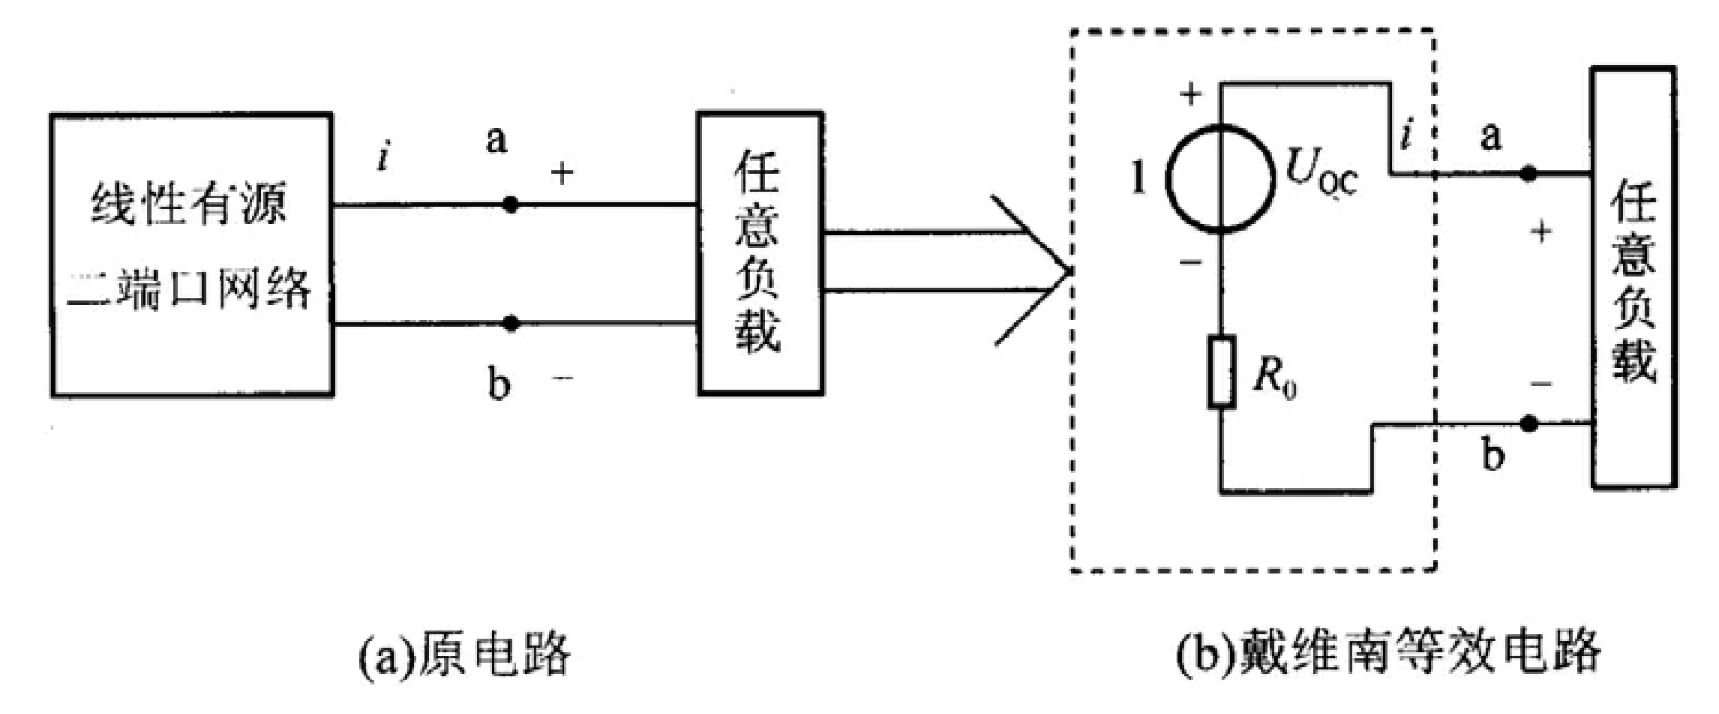
\includegraphics[width=0.5\textwidth, height=0.16\textheight]{Th_Eq.png}
    \label{fig4}
\end{figure}



诺顿定理：线性二端口电路可以用由电流源$I_{N}$和与之并联的电阻$R_{N}$构成的等效电路所取代，其中$I_{N}$为流过端口的短路电流， $R_{N}$为独立源关闭时，端口的输入电阻或等效电阻。
\begin{figure}[H]
    \centering
    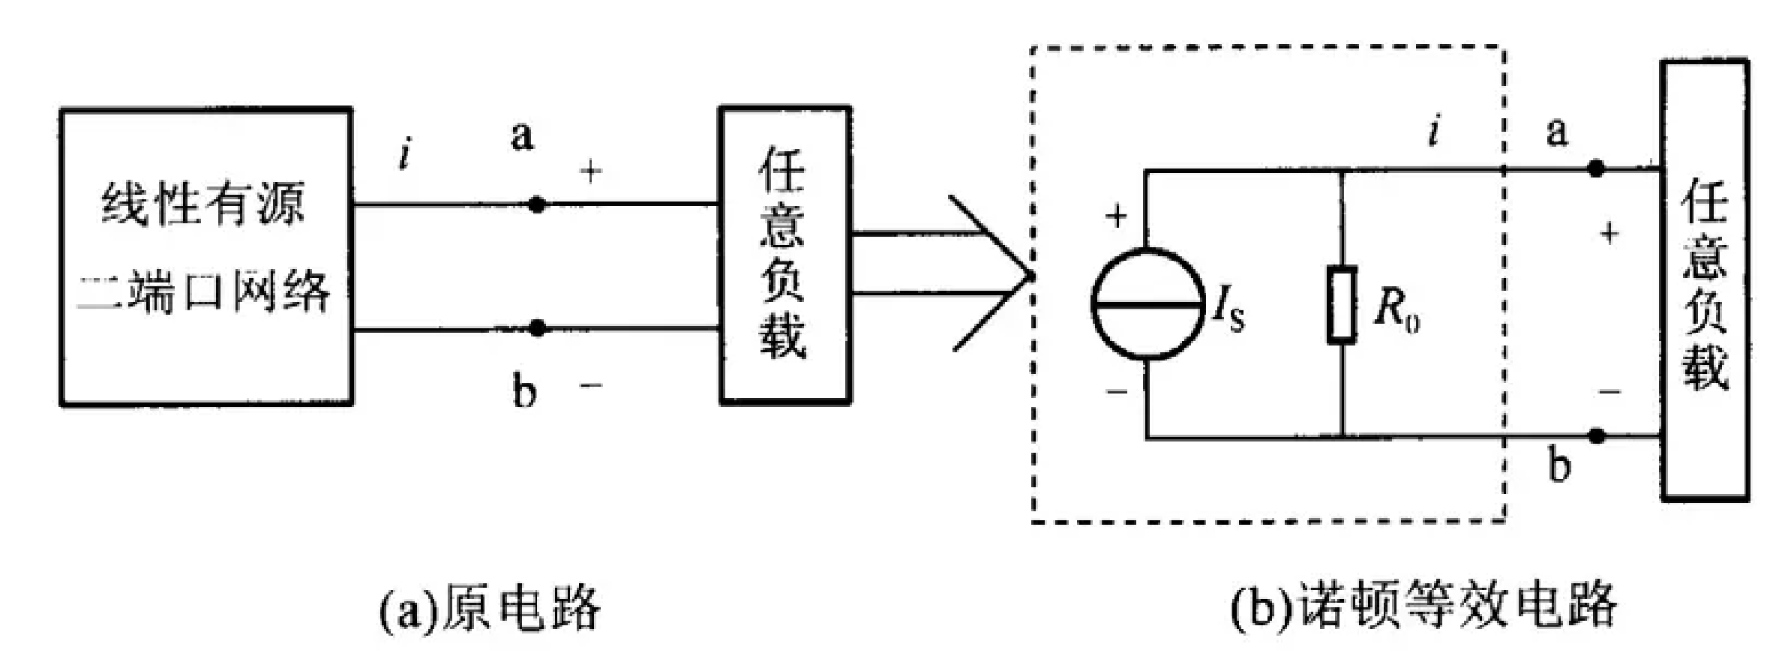
\includegraphics[width=0.5\textwidth, height=0.14\textheight]{No_Eq.png}
    \label{fig5}
\end{figure}


\section*{四、实验方案设计与参数计算}

\subsection*{4.1 实验电路}

图\ref{fig1}是验证基尔霍夫定律和叠加定理的实验电路。

\begin{figure}[H]
    \centering
    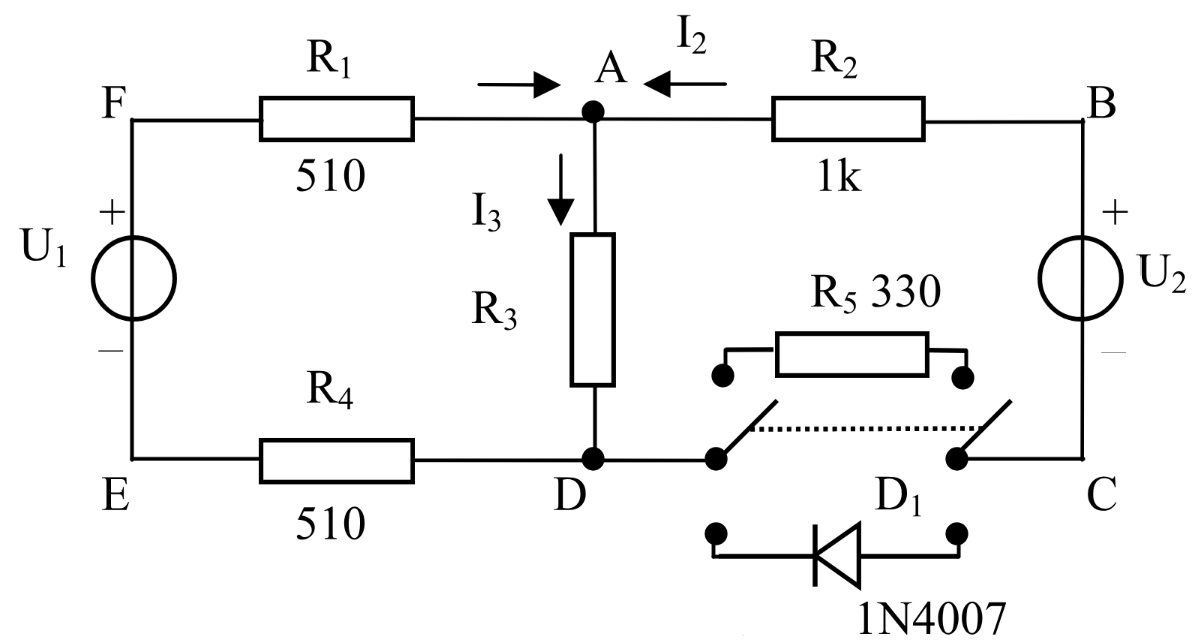
\includegraphics[width=0.4\textwidth, height=0.15\textheight]{Kichhoff.png}
    \caption{基尔霍夫定律、叠加定理实验电路}
    \label{fig1}
\end{figure}

图\ref{fig2}是验证戴维南/诺顿定理的实验电路。

\begin{figure}[H]
    \centering
    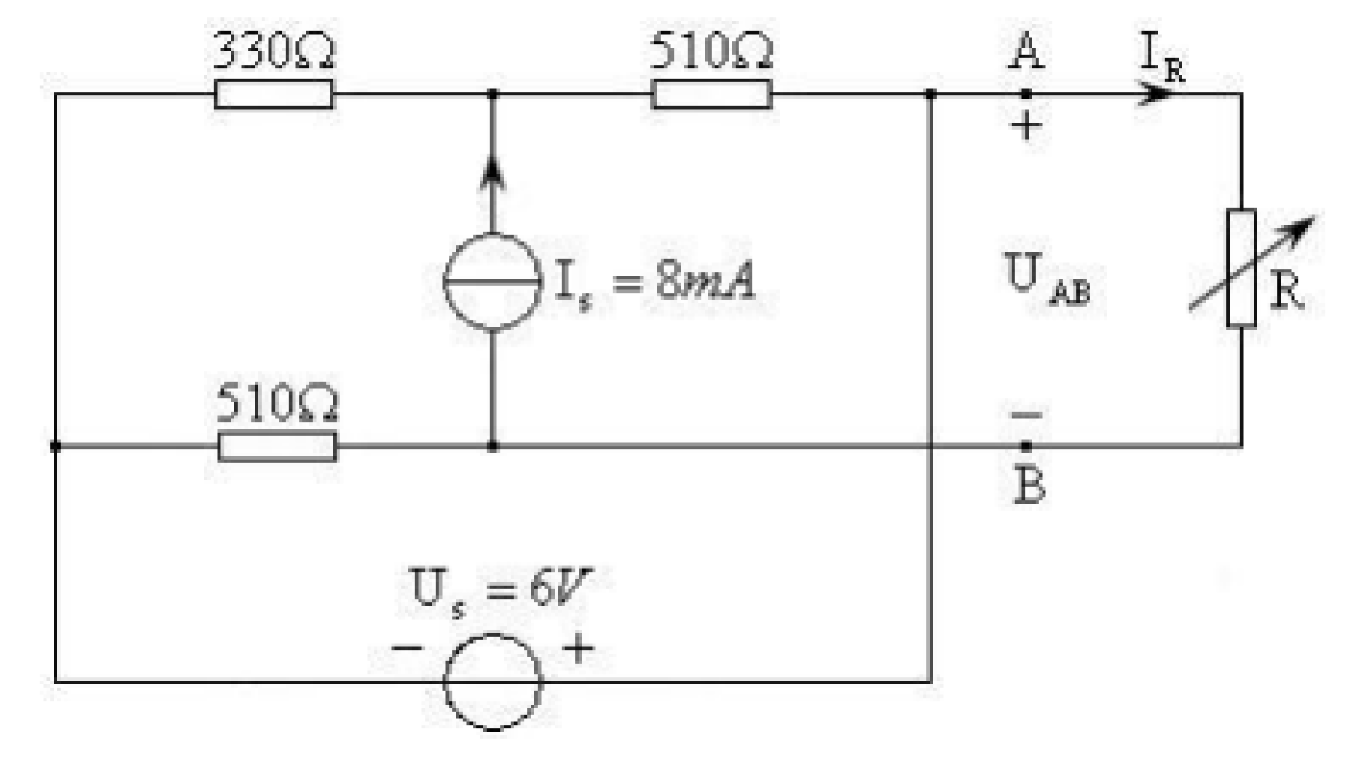
\includegraphics[width=0.4\textwidth, height=0.16\textheight]{Thevenin_Norton.png}
    \caption{戴维南/诺顿定理实验电路}
    \label{fig2}
\end{figure}

\subsection*{4.2 理论计算}

对于验证基尔霍夫定律和叠加定理的实验电路，设两回路电流$i_{1}$,$i_{2}$,方向顺时针，列写KVL方程：
$$
\left\{
\begin{aligned}
1530 i_1 - 510 i_2 &= 6 \\
-510 i_1 + 1840 i_2 &= -12
\end{aligned}
\right.
$$
解得
$$i_{1}=1.92\mathrm{mA},i_{2}=-5.99\mathrm{mA}$$

据此可得出各支路电压和各支路电路：
\begin{align*}
&I_1 = 1.76\ \mathrm{mA},   && I_2 = 5.94\ \mathrm{mA},   && I_3 = 7.78\ \mathrm{mA}, \\
&U_{FA} = -6.02\ \mathrm{V}, && U_{AB} = -1.93\ \mathrm{V}, && U_{AD} = 4.05\ \mathrm{V}, \\
&U_{CD} = 0.95\ \mathrm{V},  && U_{DE} = 1.01\ \mathrm{V}
\end{align*}

同理可求得将电阻$R_{5}$替换成二极管$D_{1}$后的各支路电压和各支路电路：
\begin{align*}
&I_1 = 3.81\ \mathrm{mA},   && I_2 = 0\ \mathrm{mA},        && I_3 = 3.81\ \mathrm{mA}, \\
&U_{FA} = 0\ \mathrm{V},     && U_{AB} = 1.98\ \mathrm{V},   && U_{AD} = -10.04\ \mathrm{V}, \\
&U_{CD} = 1.95\ \mathrm{V},  && U_{DE} = 2.07\ \mathrm{V}
\end{align*}

对于验证戴维南等效定理的实验电路，计算出戴维南等效的$V_{Th}$和$R_{Th}$，即计算电流除负载外的开路电压$U_{oc}$和等效电阻$R_{eq}$，并可得出短路电流$I_{sc}$：
$$V_{Th}=10.08\mathrm{V},R_{Th}=510\Omega,I_{sc}=19.76\mathrm{mA}$$


\section*{五、实验仪器设备}

万用表、电流表、直流稳压电源、电流源。

\section*{六、实验步骤、调试过程、实验数据记录}

\subsection*{6.1 验证基尔霍夫定律/叠加定理}


将电阻$R_{5}$接入电路，接入电压源$U_{1}=6$V,$U_{2}=12$V。用电流表测得各支路的电流值，用电压表测得各节点的电压值，并记录数据：





\begin{table}[H]
\centering
\caption{各支路电流测量值（电阻）（单位：mA）} 
\renewcommand{\arraystretch}{1.2}
\small
\begin{tabular}{|p{1.5cm}|p{1.3cm}|p{1.3cm}|p{1.3cm}|}
\hline
& $I_{1}$ & $I_{2}$ & $I_{3}$ \\
\hline
计算值 & 1.92 & 5.99 & 7.91 \\
\hline
测量值 & 1.76 & 5.94 & 7.78\\
\hline
\end{tabular}

\end{table}

\begin{table}[H]
\centering
\caption{各节点间电压测量值（电阻）（单位：V）} 
\renewcommand{\arraystretch}{1.2}
\small
\begin{tabular}{|p{1.3cm}|p{1.1cm}|p{1.1cm}|p{1.1cm}|p{1.1cm}|p{1.1cm}|p{1.1cm}|p{1.1cm}|}
\hline
& $U_{1}$ & $U_{2}$ & $U_{FA}$ & $U_{AB}$ & $U_{AD}$ & $U_{CD}$ & $U_{DE}$ \\
\hline
计算值 & 6 & 12 & 0.982 & -5.988 & 4.036 & -1.976 & 0.982 \\
\hline
测量值 &6.0 &12.0 &1.01 &-6.02 &4.05 &-1.93 &0.95 \\
\hline
\end{tabular}

\end{table}


将电阻$R_{5}$替换成二极管$D_{1}$，测量各支路电流和各元件间的电压，得到下列数据：

\begin{table}[H]
\centering
\caption{各支路电流测量值（二极管）（单位：mA）} 
\renewcommand{\arraystretch}{1.2}
\small
\begin{tabular}{|p{1.5cm}|p{1.3cm}|p{1.3cm}|p{1.3cm}|}
\hline
& $I_{1}$ & $I_{2}$ & $I_{3}$ \\
\hline
计算值 &3.92 &0 &3.92 \\
\hline
测量值 &3.81 &0 &3.81 \\
\hline
\end{tabular}

\end{table}



\begin{table}[H]
\centering
\caption{各节点间电压测量值（二极管）（单位：V）} 
\renewcommand{\arraystretch}{1.2}
\small
\begin{tabular}{|p{1.3cm}|p{1.1cm}|p{1.1cm}|p{1.1cm}|p{1.1cm}|p{1.1cm}|p{1.1cm}|p{1.1cm}|}
\hline
& $U_{1}$ & $U_{2}$ & $U_{FA}$ & $U_{AB}$ & $U_{AD}$ & $U_{CD}$ & $U_{DE}$ \\
\hline
计算值 &6 &12 &2 &0 &2 &-10 &2 \\
\hline
测量值 &6.0 &11.9 &2.07 &0 &1.98 &-10.04 & 1.98\\
\hline
\end{tabular}

\end{table}

分别令$U_{1}$,$U_{2}$单独工作，用电流表测得各支路的电流值，用电压表测得各节点的电压值，并记录数据：

\begin{table}[H]
\centering
\caption{验证叠加定理数据记录表（电阻）（单位：电压/V 电流/mA）} 
\renewcommand{\arraystretch}{1.2}
\footnotesize
\begin{tabular}{|p{2.6cm}|p{1cm}|p{1cm}|p{1cm}|p{1cm}|p{1cm}|p{1cm}|p{1cm}|p{1.0cm}|p{1cm}|p{1cm}|}
\hline
 & $U_{1}$ & $U_{2}$ & $I_{1}$ & $I_{2}$ & $I_{3}$ & $U_{FA}$ & $U_{AB}$ & $U_{AD}$ & $U_{CD}$ & $U_{DE}$ \\
\hline
$U_{1}$单独作用 &6.0 &0 &4.17 &-1.16 &3.02 &1.19 &0.38 &1.57 &2.15 &2.28 \\
\hline
$U_{2}$单独作用 &0 &12.0 &-2.32 &7.12 &4.76 &-7.22 &-2.31 &2.48 &-1.20 &-1.26 \\
\hline
$U_{1}$ $U_{2}$共同作用 &6.0 &12.0 &1.76 &5.94 &7.78 &-6.02 &-1.93 &4.05 &0.95 &1.01 \\
\hline
\end{tabular}

\end{table}

\begin{table}[H]
\centering
\caption{验证叠加定理数据记录表（二极管）（单位：电压/V 电流/mA）} 
\renewcommand{\arraystretch}{1.2}
\footnotesize
\begin{tabular}{|p{2.6cm}|p{1cm}|p{1cm}|p{1cm}|p{1cm}|p{1cm}|p{1cm}|p{1cm}|p{1.0cm}|p{1cm}|p{1cm}|}
\hline
& $U_{1}$ & $U_{2}$ & $I_{1}$ & $I_{2}$ & $I_{3}$ & $U_{FA}$ & $U_{AB}$ & $U_{AD}$ & $U_{CD}$ & $U_{DE}$ \\
\hline
$U_{1}$单独作用 &6.0 &0 &4.15 &-1.02 &3.12 &1.03 &1.63 &0.59 &2.10 &2.25 \\
\hline
$U_{2}$单独作用 &0 &11.9 &0 &0 &0 &0 &0 &-12.02 &0 &0 \\
\hline
$U_{1}$ $U_{2}$共同作用 &6.0 &11.9 &3.81 &0 &3.81 &0 &1.98 &-10.04 &1.95 &2.07 \\
\hline
\end{tabular}

\end{table}

\subsection*{6.2 验证戴维南定理}

本次实验选择验证戴维南定理。

断开负载$R_{L}$，用万用表测量其开路电压$U_{oc}$及等效电阻$R_{eq}$,并记录数据：



\begin{table}[H]
\centering
\caption{戴维南/诺顿等效电路的参数} 
\renewcommand{\arraystretch}{1.2}
\small
\begin{tabular}{|p{1.5cm}|p{1.5cm}|p{1.5cm}|}
\hline
 $U_{OC}$(V) & $I_{SC}$(mA) & $R_{O}$($\Omega$) \\
\hline
 10.07 &19.31 &520 \\
\hline


\end{tabular}

\end{table}

改变$R_{L}$阻值，使$U_{AB}$在0到$U_{oc}$之间均匀选取测量点，记录负载阻值$R_{L}$，以及负载两端电压$U_{R_{L}}$（即$U_{AB}$）和流经负载电流$I_{R_{L}}$：

\begin{table}[H]
\centering
\caption{二端口网络外特性（实验电路）} 
\renewcommand{\arraystretch}{1.2}
\small
\begin{tabular}{|p{1.5cm}|p{1.5cm}|p{1.5cm}|p{1.5cm}|}
\hline
 $R_{L}$($\Omega$)& 523 & 1012 & 2035 \\
\hline
$U_{AB}$(V) & 4.85 & 6.72 & 8.15\\
\hline
$I$(mA) & 9.25 & 6.65 & 4.01\\
\hline
\end{tabular}
\end{table}




利用刚才测得的开路电压$U_{oc}$和等效电阻$R_{eq}$，构建戴维南等效电路：电流源$U_{S}=U{oc}$,电阻$R_{o}=R_{eq}$。

改变$R_{L}$阻值，使$U_{AB}$在0到$U_{oc}$之间均匀选取测量点，记录负载阻值$R_{L}$，以及负载两端电压$U_{R_{L}}$（即$U_{AB}$）和流经负载电流$I_{R_{L}}$：





\begin{table}[H]
\centering
\caption{二端口网络外特性（戴维南等效电路）} 
\renewcommand{\arraystretch}{1.2}
\small
\begin{tabular}{|p{1.5cm}|p{1.5cm}|p{1.5cm}|p{1.5cm}|}
\hline
 $R_{L}$($\Omega$)& 169 & 730 & 1463 \\
\hline
$U_{AB}$(V) & 23.41 & 5.83 & 7.40\\
\hline
$I$(mA) & 14.26& 7.96 & 5.03\\
\hline


\end{tabular}

\end{table}

绘制等效电路二端口网络外特性的$U-I$曲线，并标记实验测得的数据点：

\begin{figure}[H]
    \centering
    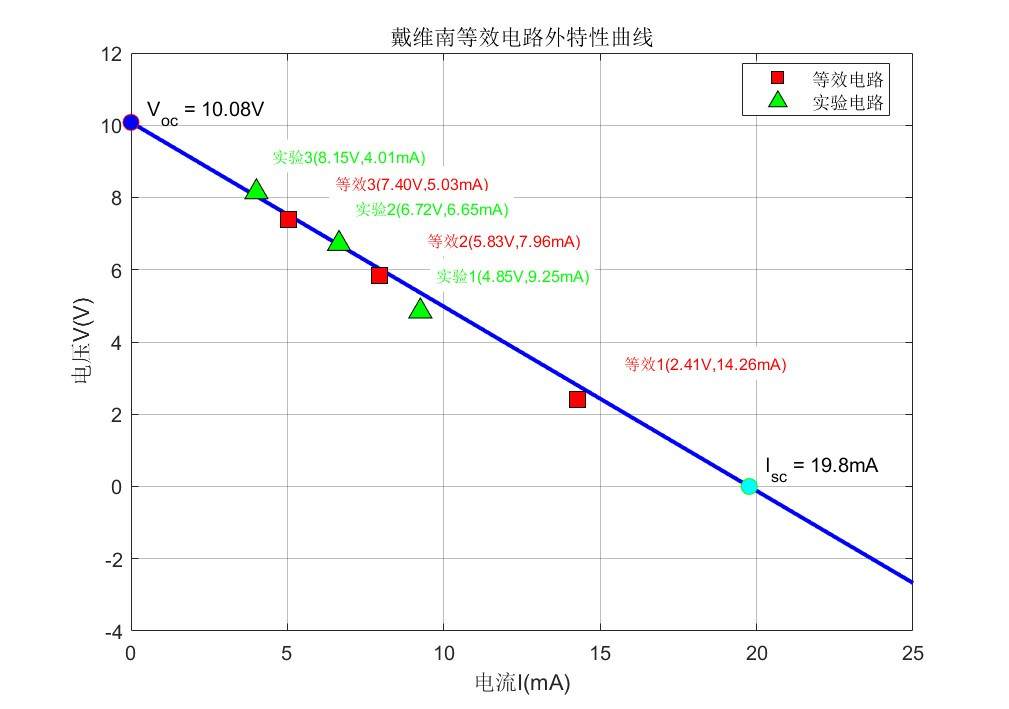
\includegraphics[width=0.6\textwidth, height=0.3\textheight]{Thevenin.jpg}
    \caption{戴维南等效电路二端口网络外特性}
    \label{fig3}
\end{figure}



\section*{七、数据分析与讨论}

验证基尔霍夫定律时，测量值和理论值非常接近，特别是二极管$D_{1}$接入时$I_{2}$理论值和测量值均为0，验证了基尔霍夫定律的普适性（对非线性电路也成立）。

验证叠加定理时，将电阻$R_{5}$接入电路时，第三列数据基本等于第一列数据与第二列数据数据之和，由此可以验证叠加定理。

但是二极管$D_{1}$接入电路时，$U_{1}$单独作用时，$I_{2}> 0$,可能是由于二极管存在漏电流。此时只满足$$I_{1}+I_{2}=I_{3}$$但是$$I_{U_{1}}+I_{U_{2}}\neq I_{U_{1}+U_{2}}$$

这就说明对于非线性电路，基尔霍夫定律成立，而（线性）叠加定理是不成立的。

验证戴维南等效定理时，测量得到的等效参数和理论计算值相符合。实验测得的实验电路和等效电路二端口网络外特性的数据点和理论值$U-I$曲线相吻合，说明戴维南等效电路能够实现等效效果，从而验证戴维南定理。

当然其中也存在着一些问题，比如测量获得的数据点数量过少，以及数据点未能够均匀分布，等等，这样还是会欠缺一些说服力的。


实验时的测量值与理论值存在误差，但这种测量误差是不可避免的。不过这种误差在可接受范围内，说明实验方法和实验设备准确性较高。

\section*{八、结论}

1、成功验证了基尔霍夫电流定律和基尔霍夫电压定律。

2、成功验证了叠加定理。

3、成功验证了戴维南等效定理。

\section*{九、心得与体会}

1、课前要做好实验的准备工作，为实验数据记录打好表格，同时要对实验操作和过程做到心中有数。

2、在调整电路之前要断开电源。

3、针对电流源，要确保其电量充足或外接供电。本次实验验证戴维南等效时，接入电源后对实验电路测量，发现与理论值差距过大。在排查期间，电流表没电了，在外接供电后再进行测量，终于和理论值相吻合，从而继续后面的测量。

4、实验中要测量记录的数据很多，就特别需要耐心和细心。

\section*{十、思考题}

1、如果设定不同的电压与电流参考方向，基尔霍夫定律是否仍然成立？

答：基尔霍夫定律描述的是电压/电流的代数和为0，这和参考方向的选取无关。参考方向的不同只会改变最终求得数值的正负号。

2、如果电路中含有非线性器件，基尔霍夫定律是否仍然成立？

答：KCL的实质是电荷守恒，KVL的实质是能量守恒，是普适的，和电路是不是线性的没有关系。

3、可否直接将不起作用的电源（$U_{1}$或$U_{2}$）短接置零？

答：虽然在理论上要将电压源短接，但这会导致电压源承受巨大的电流，从而烧坏电源。（虽然实验使用的直流稳压源有保护功能，但像干电池就完全不能保护，所以养成良好习惯，不要短接电压源！）

4、根据测量数据，计算各种状况下，某一电阻消耗的功率，并验证功率是否具有叠加性。

答：我们计算将电阻$R_{5}$接入电路时，电阻$R_{3}$的功率。

\begin{table}[H]
\centering

\renewcommand{\arraystretch}{1.2}
\footnotesize
\begin{tabular}{|p{2.6cm}|p{1cm}|p{1cm}|p{1cm}|}
\hline
 & $I_{3}$  & $U_{AD}$ & $P$   \\
\hline
$U_{1}$单独作用  &3.02  &1.57 &4.74  \\
\hline
$U_{2}$单独作用  &4.76  &2.48 &11.80  \\
\hline
$U_{1}$ $U_{2}$共同作用 &7.78  &4.05 &31.51  \\
\hline
\end{tabular}

\end{table}

可以发现$P_{1}+P_{2}\neq P$，所以功率不具有叠加性。

在数学上，若$i=i_{1}+i_{2},u=u_{1}+u_{2}$,则$p_{1}=u_{1}i_{1},p_{2}=u_{2}i_{2}$，而
$$p=ui=(u_{1}+u_{2})(i_{1}+i_{2})=u_{1}i_{1}+u_{2}i_{2}+u_{1}i_{2}+u_{2}i_{1}=p_{1}+p_{2}+...\neq p_{1}+p_{2}$$
理论和实验都证明，功率不具有叠加性。

5、在求戴维南或诺顿等效电路时，做短路实验，则测$I_{sc}$的条件是什么?在本实验中可否直接做负载短路实验?

答：（1）断开负载和电路的连接，将二端口用导线（杜邦线）相连。要求 AB 端的等效电阻应该足够大，否则流经电源的电流过大会损坏电源。

（2）直接对负载短路，会产生远超电路设计值的巨大电流，超过电源允许最大值，电源可能被烧坏！

6、简述测量有源二端口网络开路电压及等效内阻的几种方法，并比较其优缺点。 

答：见下表。
\begin{table}[H]
\centering
\label{tab:method_comparison}
\renewcommand{\arraystretch}{1.5}
\footnotesize
\begin{tabular}{|p{1.8cm}|p{4.5cm}|p{3.2cm}|p{3.2cm}|}
\hline
\textbf{测量方法} & \textbf{核心操作与原理} & \textbf{优点} & \textbf{缺点} \\
\hline
\textbf{直接测量法} & 
\textbf{开路电压} \( U_{oc} \)：直接用高内阻电压表测量输出端电压。\newline
\textbf{等效内阻} \( R_o \)：无法直接测量，需结合其他方法（如伏安法）计算。
& 
\begin{minipage}[t]{\linewidth}
测量\(U_{oc}\)的原理和操作极为简单、直观。
\end{minipage}
& 
\begin{minipage}[t]{\linewidth}
若电压表内阻不够高，会引入较大误差，测得的\(U_{oc}\)小于真实值。\\
无法直接得到\(R_o\)。
\end{minipage} \\
\hline
\textbf{开路短路法} & 
\textbf{开路电压} \( U_{oc} \)：用电压表直接测量。\newline
\textbf{短路电流} \( I_{sc} \)：用电流表将输出端短接后测量。\newline
\textbf{计算内阻：} \( R_o = \frac{U_{oc}}{I_{sc}} \)
& 
\begin{minipage}[t]{\linewidth}
原理简单，计算方便。\\
无需使用可变负载。
\end{minipage}
& 
\begin{minipage}[t]{\linewidth}
危险性强，如果网络内阻很小，短路电流\(I_{sc}\)会非常大，极易烧毁内部元件或电源。\\
仅适用于内阻较大且允许短路的网络。
\end{minipage} \\
\hline
\textbf{伏安法（外接负载法）} & 
在输出端接一个可变负载电阻\(R_L\)，测量两组或以上不同的负载电压\(U_L\)和电流\(I_L\)值。\newline
\textbf{原理：} \( U_L = U_{oc} - I_L \cdot R_o \)\newline
通过列方程或作图拟合直线，其纵截距为\(U_{oc}\)，斜率为\(-R_o\)。
& 
\begin{minipage}[t]{\linewidth}
安全可靠，无需短路网络。\\
通过多次测量取平均或拟合，可以减小随机误差，精度较高。\\
能直观显示网络的输出特性。
\end{minipage}
& 
\begin{minipage}[t]{\linewidth}
操作和计算相对繁琐，需要多次测量。\\
作图法会引入人为读数误差。
\end{minipage} \\
\hline
\textbf{半电压法} & 
\textbf{第一步：}测量开路电压\(U_{oc}\)。\newline
\textbf{第二步：}接入一个可变电阻箱作为负载\(R_L\)，调节其阻值，使负载两端的电压\(U_L\)降至\(U_{oc}\)的一半，即\(U_L = \frac{U_{oc}}{2}\)。\newline
\textbf{结论：}此时负载电阻箱的阻值即为等效内阻\(R_o\)。
& 
\begin{minipage}[t]{\linewidth}
精度高：只需判断电压是否为一半，避免了电表内阻引起的系统误差。\\
安全，无需短路。\\
计算极其简单（\(R_o = R_L \mid_{U_L=U_{oc}/2}\)）。
\end{minipage}
& 
\begin{minipage}[t]{\linewidth}
需要一个精度较高且可调的数字电源或一个精密的可调电阻箱。\\
对于等效内阻非常小的网络，可能需要大功率负载。
\end{minipage} \\
\hline
\end{tabular}
\end{table}

\end{document}